\section{MUMPS: Process Pinning}
\label{subseq:mm-mumps-process-pinning}

Due to intensive and complex manipulations with frontal and and contribution matrices, we can assume that MUMPS belongs to memory bound applications. In this case memory access can be a bottleneck for the library. A common way to improve performance of memory bound applications running on distributed memory machines is to distribute processes equally among sockets of a node.\\


However, because MUMPS uses both task and data parallelism as well as a complex hybrid, both static and dynamic, task scheduling, it becomes difficult to decide which pinning strategy is better i.e. \textit{close} or \textit{spread}, described in section \ref{subseq:matrix-sets-and-hardware}.\\


Therefore, a couple of tests were conducted with both GRS and SuiteSparse matrix sets in order to investigate influence of different strategies on MUMPS performance. For this group of tests, only MUMPS default settings together with a specific fill-in reducing algorithm for each test case, mentioned in section \ref{subseq:fill-in-reordering}, were used. The tests were performed on HW1 machine using only flat-MPI mode. Results are shown in figures \ref{fig:mumps-close-vs-spread-1}, \ref{fig:mumps-close-vs-spread-2}, \ref{fig:mumps-close-vs-spread-3} and in appendix \ref{app:mm-mumps-process-pinning}. The graphs depict the total time spent, i.e. analysis, factorization and solution.\\

\figpointer{\ref{fig:mumps-close-vs-spread-1}}
\begin{figure}[htpb]
\centering
	\begin{tabular}{cc}
	\subfloat[HW1 - pwr-3d]{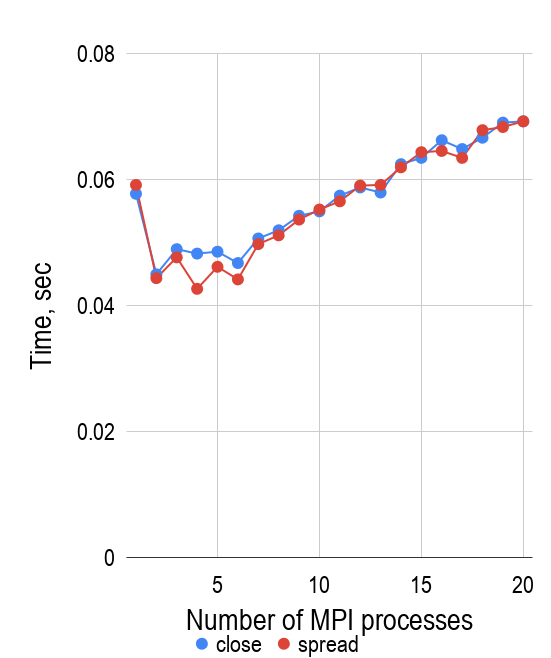
\includegraphics[width=0.48\textwidth]{figures/chapter-2/spread-vs-close/grs-cluster/pwr-3d.png}} &
		\subfloat[HW2 - pwr-3d]{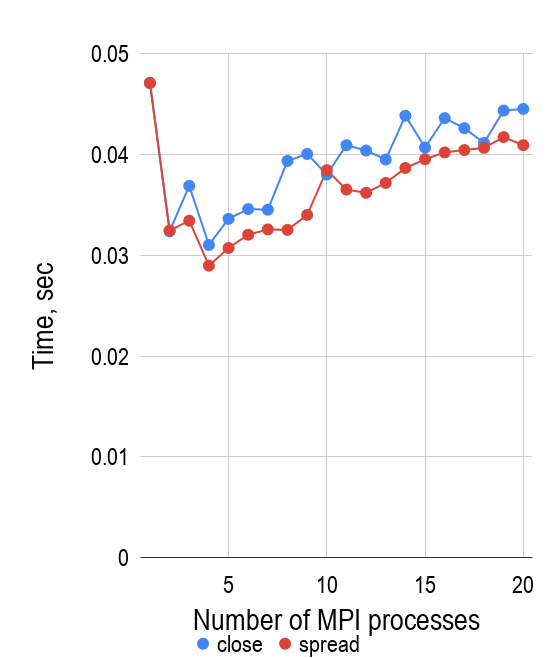
\includegraphics[width=0.48\textwidth]{figures/chapter-2/spread-vs-close/linux-cluster/pwr-3d.png}} \\
		\subfloat[HW1 - cube-64]{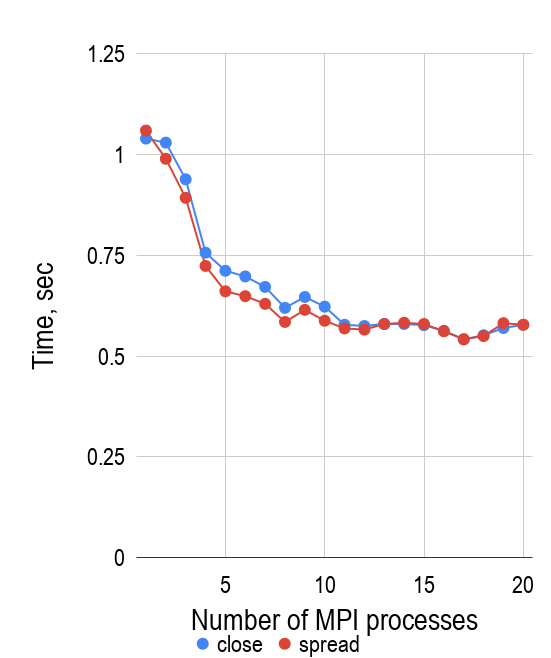
\includegraphics[width=0.48\textwidth]{figures/chapter-2/spread-vs-close/grs-cluster/cube-64.png}} &
		\subfloat[HW2 - cube-64]{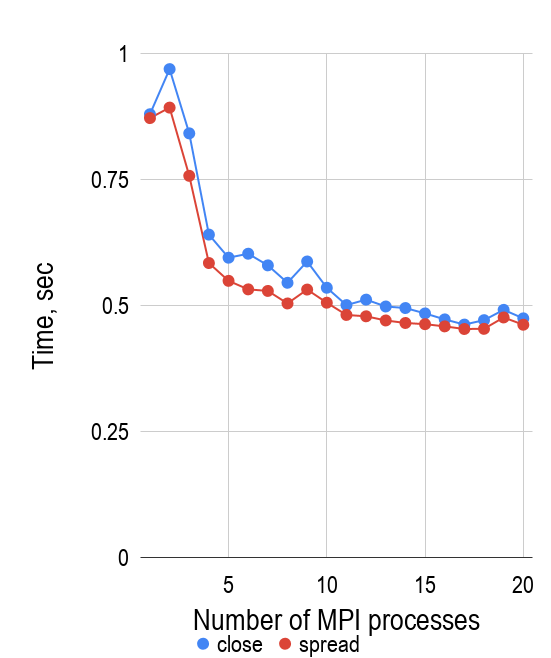
\includegraphics[width=0.48\textwidth]{figures/chapter-2/spread-vs-close/linux-cluster/cube-64.png}} \\
	\end{tabular}
	\caption{Comparison of \textit{close} and \textit{spread} pinning strategies}
	\label{fig:mumps-close-vs-spread-1}
\end{figure}



\figpointer{\ref{fig:mumps-close-vs-spread-2}}
\begin{figure}[htpb]
\centering
	\begin{tabular}{cc}
		\subfloat[HW1 - cube-645]{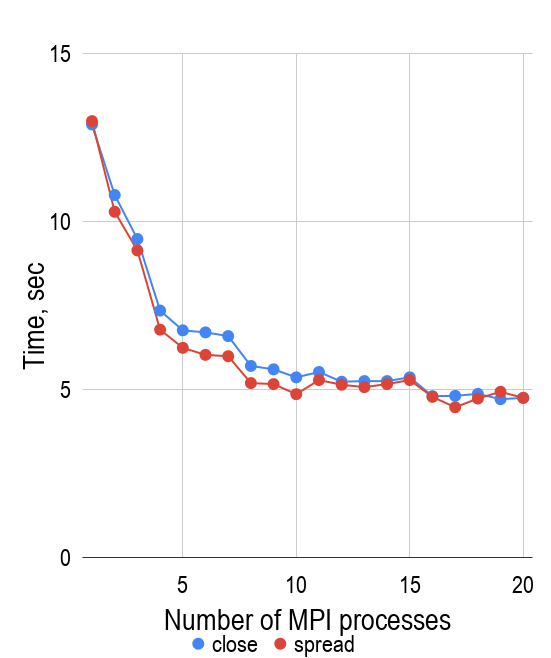
\includegraphics[width=0.48\textwidth]{figures/chapter-2/spread-vs-close/grs-cluster/cube-645.png}} &
		\subfloat[HW2 - cube-645]{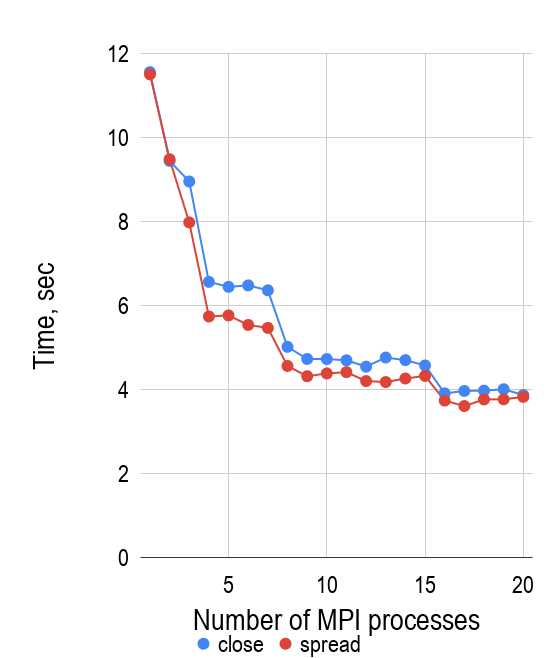
\includegraphics[width=0.48\textwidth]{figures/chapter-2/spread-vs-close/linux-cluster/cube-645.png}} \\
		\subfloat[HW1 - k3-18]{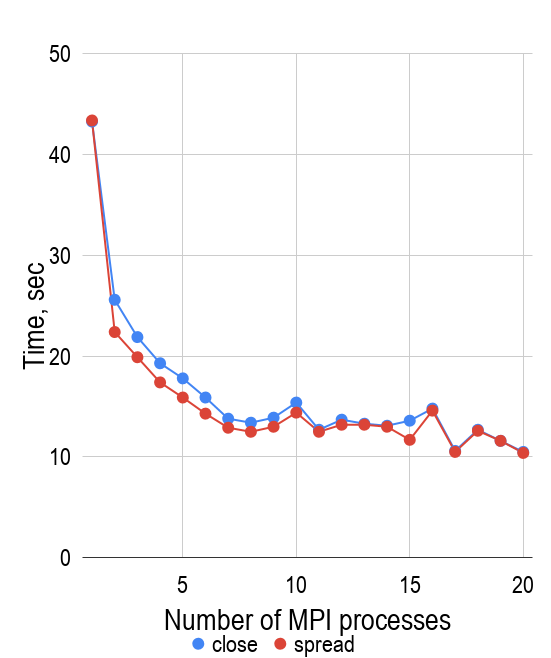
\includegraphics[width=0.48\textwidth]{figures/chapter-2/spread-vs-close/grs-cluster/k3-18.png}} &
		\subfloat[HW2 - k3-18]{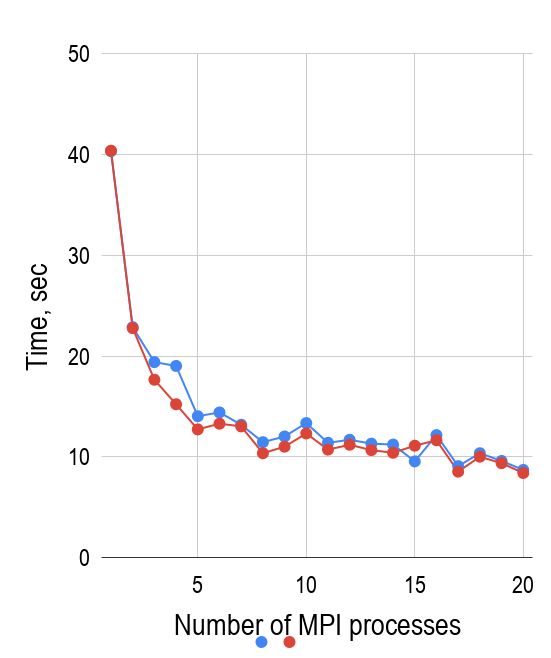
\includegraphics[width=0.48\textwidth]{figures/chapter-2/spread-vs-close/linux-cluster/k3-18.png}} \\
	\end{tabular}
	\caption{Comparison of \textit{close} and \textit{spread} pinning strategies}
	\label{fig:mumps-close-vs-spread-2}
\end{figure}




\figpointer{\ref{fig:mumps-close-vs-spread-3}}
\begin{figure}[htpb]
\centering
	\begin{tabular}{cc}
		\subfloat[HW1 - PFlow\_742]{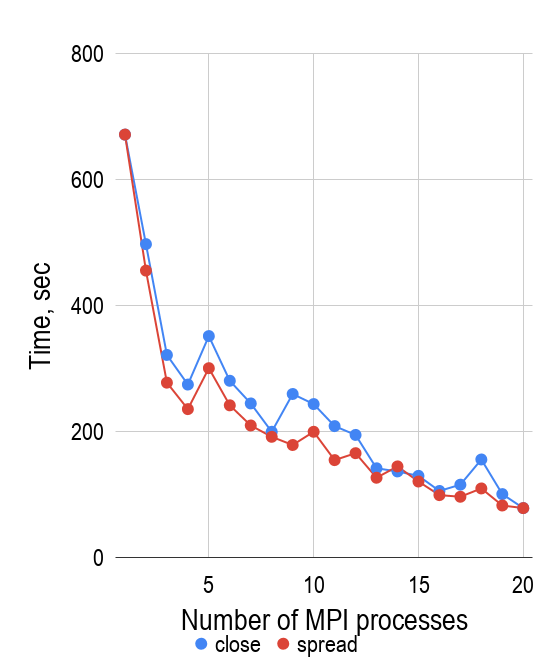
\includegraphics[width=0.48\textwidth]{figures/chapter-2/spread-vs-close/grs-cluster/PFlow_742.png}} &
		\subfloat[HW2 - PFlow\_742]{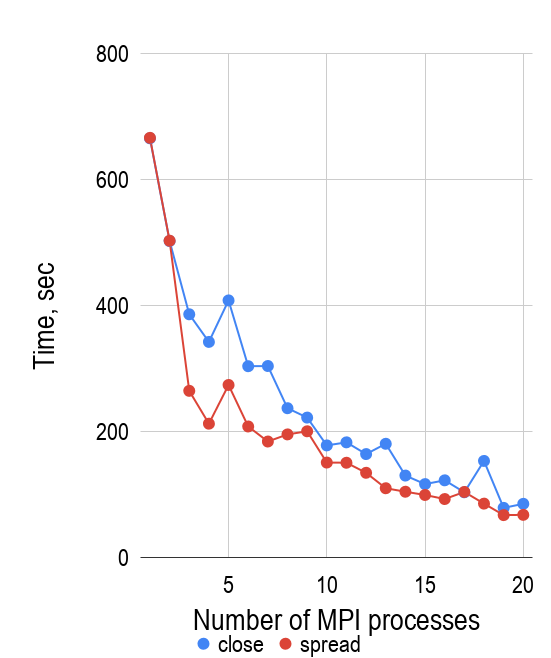
\includegraphics[width=0.48\textwidth]{figures/chapter-2/spread-vs-close/linux-cluster/PFlow_742.png}} \\
		\subfloat[HW1 - CurlCurl\_3]{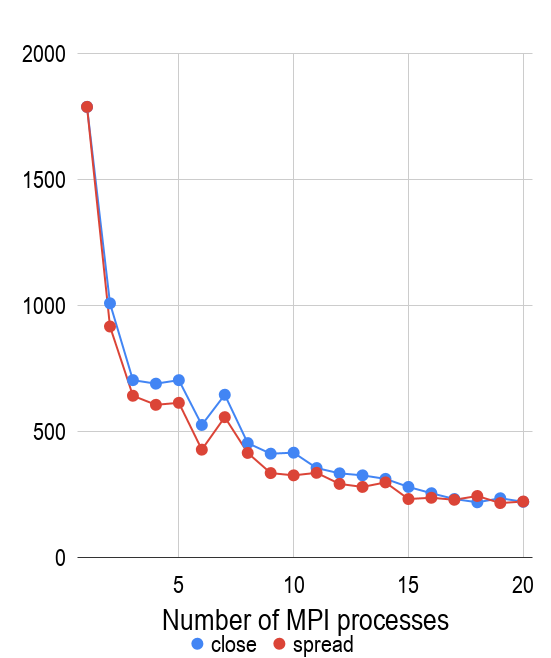
\includegraphics[width=0.48\textwidth]{figures/chapter-2/spread-vs-close/grs-cluster/CurlCurl_3.png}} &
		\subfloat[HW2 - CurlCurl\_3]{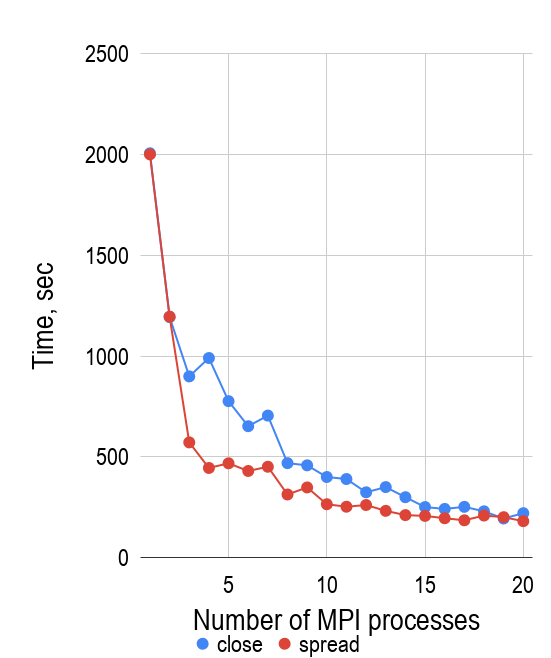
\includegraphics[width=0.48\textwidth]{figures/chapter-2/spread-vs-close/linux-cluster/CurlCurl_3.png}} \\
	\end{tabular}
	\caption{Comparison of \textit{close} and \textit{spread} pinning strategies}
	\label{fig:mumps-close-vs-spread-3}
\end{figure}


The tests revealed that \textit{spread}-pinning performed better and allowed to reduce run-time by approximately BRA\% in average in contrast to the \textit{close} strategy. As expected, the points with 1 and 20 MPI processes show the same performance because they basically represent the same process distribution. Additionally, almost BRA\% improvement can be observed around the saturation point in case of \textit{spread} strategy application.\\


Taken into account results of the tests, \textit{spread}-pinning has been chosen for the rest of the study because it shows better overall performance in the intermediate range, in terms of the number MPI processes, where a saturation point can occur. As an example, we would like to point out this process distribution can be particular useful for matrices such as \textit{pwr-3d} and \textit{cube-5} where saturation happens at the number of processes equal to 4.\\


In general, such process distribution can be easily achieved by means of some advanced OpenMPI options, for example \textit{--map-by}, as following:. \\

\begin{lstlisting}[language=bash, caption={An example of \textit{spread}-pinning with using OpenMPI options in case of a flat-MPI run}, frame=single, label={lst:iterative-refinement}]
mpiexec --map-by socket -n $num_proc $executable_name $parameters
\end{lstlisting}
